\newpage
\section{Elementary Definitions}

\subsection{Independent sets}

We will begin with the first possible way of defining what a \textit{matroid} is. This way is arguably the simplest one because the properties are intuitive and not hard to visualize. When speaking about matroids, we will always deal with finite sets, and the way we obtain a matroid from a finite set is to select some special selection of its subsets.  These special sets correspond to the \textit{independent} sets, and should obey some distinctive properties. This idea is precisely what the following definition is about.

\begin{defn}
    Let $E$ be a finite set, possibly empty, and $\mathcal{I}$ a collection of subsets of $E$ (i.e. some subset of the power set $2^E$ of E). We call the ordered pair $M = (E, \mathcal{I})$ a matroid if the following three properties are satisfied

    \begin{enumerate}
        \item[(I1)] We have $\emptyset \in \mathcal{I}$.
        
        \item[(I2)] If $I \in \mathcal{I}$ and $J \subseteq I$, then $J \in \mathcal{I}$.
        
        \item[(I3)] If $J, I \in \mathcal{I}$ and $|J| < |I|$, then there exists $e \in I - J$ so that $J \cup e \in \mathcal{I}$.
    \end{enumerate}

    We call elements of $\mathcal{I}$ \textbf{independent sets}. 
\end{defn}

There are some alternatives to the third property that are equivalent, for example we could alternatively write

\begin{enumerate}
    % The `\ ` is the hackiest thing ever, please ignore it :/
    \item [(3.*)$\ $] \textit{ If $I, J \in \mathcal{I} $ and $|J| = |I| + 1$, then there exists $e \in J - I$ such that $I \cup e \in \mathcal{I}$.}
\end{enumerate}

or

\begin{enumerate}
\item[(3.**)] \textit{If $X \subseteq E$ and $I_1, I_2$ are maximal members of $\{ I \in \mathcal{I} | I \subseteq X \}$, then $|I_1| = |I_2|$.}
\end{enumerate}

\begin{exmp}
In  figure~\ref{fig:1234-matroid-independent-sets} we find a representation of a matroid by writing all subsets of the ground set $\{1,2,3,4\}$ and coloring them accordingly. The independent sets are colored in orange. It is clear that the empty set is independent and that all subsets of independent sets are independent. The dependent sets, colored in cyan, are the sets that are not independent.
\end{exmp}


\begin{figure}[h]

\begin{center}
\begin{tikzpicture}

\matrix (a) [matrix of math nodes, column sep=0.6cm, row sep=0.6cm,]{
 & & &\textcolor{cyan}{
1234} & & & &\\
 \textcolor{cyan}{
123}& &\textcolor{cyan}{
124} & &\textcolor{cyan}{
134} &  & \textcolor{cyan}{
234}  \\
\textcolor{orange}{12} & \textcolor{cyan}{13} & \textcolor{cyan}{14} & & \textcolor{orange}{23} & \textcolor{cyan}{
24} & \textcolor{cyan}{
34} \\
\textcolor{orange}{1}& &\textcolor{orange}{2} & & \textcolor{orange}{3}& & \textcolor{cyan}{4} \\
& & & \textcolor{orange}{\emptyset} &  & & \\
&&&&&& \\};

\foreach \i/\j in {1-4/2-1, 1-4/2-3, 1-4/2-5, 1-4/2-7, 2-1/3-1, 2-1/3-2, 2-1/3-5, 2-3/3-1, 2-3/3-3, 2-3/3-6, 2-5/3-2, 2-5/3-3, 2-5/3-7, 2-7/3-5, 2-7/3-6, 2-7/3-7, 3-1/4-1, 3-1/4-3, 3-2/4-1, 3-2/4-5, 3-3/4-1, 3-3/4-7, 3-5/4-3, 3-5/4-5, 3-6/4-3, 3-6/4-7, 3-7/4-7, 3-7/4-5, 4-1/5-4, 4-3/5-4, 4-5/5-4, 4-7/5-4}
\draw[double, line width = 0.005mm, color = brown] (a-\i) -- (a-\j);

\node[draw] at (0, -2.5){\small \textcolor{orange}{Independent set}, \textcolor{cyan}{Dependent set}};

\end{tikzpicture} % why does it say this??? Did you forget a semicolon?
\end{center}
\caption{Diagram of a 4-element matroid, with dependent and independent sets colored accordingly.}
\label{fig:1234-matroid-independent-sets}
\end{figure}


The definition of a matroid is designed to extract out the property that makes a subset of elements 'independent'. This leads us to our first examples, namely the so-called \textit{representable matroids} arising from linear algebra. We say that a subset of vectors is \textit{independent} in a matroid, if and only if it is \textit{linearly independent} in the usual sense. 
%This means, in particular, that the subsets have the same properties.



 Let $A \in \mat_{m \times n}(\mathbb{F})$ where $\mathbb{F}$ is a field. In the article we will not just be interested with $\mathbb{F} = \mathbb{C} \; \mathrm{or}\; \mathbb{F} = \mathbb{R} $ but also in finite fields\footnote{In particular, we are interested in $\mathbb{Z} / p\mathbb{Z}$. By that we mean $\mathbb{Z}$ modulo $p\mathbb{Z}$ so the set of reminders when dividing by a prime number $p$. We will denote this field by $\mathbb{F}_p$}.

\begin{exmp}
    

 
 We will pick a concrete example of $A \in  \mat_{3 \times 4}(\mathbb{R})$ to illustrate that the set of columns of a matrix has a natural matroid structure. Suppose

$$A = \begin{pmatrix}

2 & 0 & 2 & 0 \\
1 & -1 & 0 & 0 \\
0 & 3 & 3 & 0


\end{pmatrix}.$$

We would like to consider \textit{the set of labels of columns of the matrix $A$} and form a matroid on it. This means we start with $E = \{1,2,3,4\}$ so a finite set where the number $1$ corresponds to the column $\begin{pmatrix} 2 & 1 & 0 \end{pmatrix} ^ T$, the number 2 corresponds to $\begin{pmatrix}  0 & -1 & 3  \end{pmatrix} ^ T$ and so forth. We now declare that a subset of $E$ is called independent if and only if the corresponding set of column vectors is linearly independent as a set of vectors in $\mathbb{R}^3$. We can explicitly check what this means in our example. The sets $\{1\}$, $\{2\}$, $\{3\}$ are all independent because they correspond to non-zero vectors. For the two-element subsets we see that $\{1,2\}$, $\{1,3\}$ and $\{2,3\}$ are all independent, while any two element subsets containing the last column are not. Finally, the 3-element subset $\{1,2,3\}$ is not independent because as vectors, the first and the second column sum up to the third. So to conclude, the collection of all independent sets is
$$\mathcal{I} = \{\emptyset, \{1\}, \{2\}, \{3\}, \{1,2\}, \{1,3\}, \{2,3\} \},$$

which indeed satisfies the properties of collection of independent sets of a matroid. This is not a coincidence, we will prove that a collection of subsets formed from a matrix in the above way is always a matroid.

\end{exmp}


\begin{theorem}

    Let $A \in \mathrm{Mat} _{m \times n}(\mathbb{F})$ and $E = \{1, 2, \cdots, n\}$ be a finite set of $n$ elements where the element $i$ corresponds to the $i$-th column of the matrix $A$. We call a subset $I \subseteq E$ independent if and only if the column vectors that the members of $I$ correspond to form a linearly independent set as members of $\mathbb{F}^n$, and denote the collection of all independent subsets as $\mathcal{I}$. Then $M = (M, \mathcal{I})$ is a matroid, and we denote it by $M[A]$.
    
\end{theorem}

\begin{proof}
    We need to check that the collection $\mathcal{I}$ satisfies the three properties for the collection of independent sets given in the definition. 

\begin{enumerate}

    \item[(I1)] First, $\emptyset$ is trivially in $\mathcal{I}$.
    
    \item[(I2)] The second property is also satisfied because if $J \subseteq I$ and $I \in \mathcal{I}$ this means that the vectors corresponding to $I$ form a linearly independent set. In particular, let $v_1, v_2, \cdots v_j, v_{j+1}, \cdots v_{i}$ be the column vectors corresponding to $I$, and that first $j$ are also in $J$, that means $|I| = i$, $|J| = j$ and $j \leq i$. If for some linear combination we have $a_1v_1 + \cdots + a_jv_j = 0$, where $a_i \in \mathbb{F}$ then it is also true that $a_1v_1 + \cdots + a_jv_j + 0 \cdot a_{j+1} + \cdots + 0 \cdot a_i = 0$. Since the vectors of $I$ are linearly independent it now follows that $a_1 = a_2 = \cdots a_j = 0$ as well. So the vectors corresponding to the elements of $J$ are also linearly independent, which means by definition $J \in \mathcal{I}$.

    \item[(I3)] Finally, we have to check third property. We assume that $J, I \in \mathcal{I}$ and $|J| < |I|$. We denote by $V_J$ and $V_I$ the linear subspaces of $\mathbb{F}^n$ spanned by vectors corresponding to $J$ and $I$ respectively. Because the vectors corresponding to $J$ and $I$ are linearly independent, they also form a basis for $V_J$ and $V_I$ respectively. For any $e \in I - J$ we denote by $v(e) \in \mathbb{F}^n$ the column vector of $A$ corresponding to $e$. Suppose some $e \in I - J$ has the property that adding it to $J$ does not change the dimension of the subspace spanned by J, i.e. $\dim (V_J \cup v(e)) = \dim (V_J) = |J|$. Then $v(e)$ is already in $V(J)$ because the vectors corresponding to $J$ are linearly independent and if the dimension does not increase, then $v(e)$ can be expressed as a linear combination of vectors corresponding to $J$. However, this cannot hold true for \textit{every} $e \in I - J$. Suppose for contradiction, that for every $e \in I - J$ it holds that the vector $v(e) $ is already in $ V_J$. Because for all elements in the intersection,  $i \in I \cap J$, we have $v(i) \in V_J$ by definition, we could then infer $V_I \subseteq V_J$. But this implies that 

    $$|I| = \dim(V_I) = \dim(V_J) = |J| < |I|$$
     which is a contradiction. So there is at least one $e \in I - J$ so that $\dim(V_J \cup v(e)) = \dim(V_J) + 1$, which means the vectors corresponding to $J \cup e$ form a linearly independent subset. Finally, this means that $J \cup e \in \mathcal{I}$ which proves the third property.

\end{enumerate}
\end{proof}

In order to talk about any classification of matroids we have to say when the two matroids are equivalent - representing the same structure of independent sets. Intuitively, it is nothing deep, the definition will just rephrase that the two are \textit{equal} if it is possible to relabel the elements of the first matroid to the elements of the second without changing the independent sets.

\begin{defn}
    We call two matroids $M = (E, \mathcal{I})$ and $N = (F, \mathcal{J})$ isomorphic and denote it by $M \sim N$ if there exists a bijection $f: E \to F$ so that a subset $K \subseteq F$ is independent if and only if $K = f(L)$ for some independent set $L \in \mathcal{I}$.
\end{defn}


\begin{defn}
    We call a matroid $M$ representable, if $M$ is isomorphic to a matrix matroid $N[A]$ for some $A \in \mat_{m \times n}(\mathbb{F})$ over some field $\mathbb{F}$. Moreover, we  call it $\mathbb{F}$-representable if it is representable over specific field $\mathbb{F}$.
\end{defn}

We will now define another important class of matroids. Due to its simplicity it will be suitable as an example in many of the notions defined in the proceeding text.

\begin{defn}\label{uniformM}
    Let $E = \{1, 2, \cdots, n\}$ and $\mathcal{I} = \{ L \subseteq E \; \text{ such that } \; |L| \leq m\}$. Then $(E, \mathcal{I})$ is a matroid which we denote by $U_{m,n}$ and call it a uniform matroid of rank $m$ on a $n$ element set.
\end{defn}
\begin{theorem}
    The ordered pair $U_{m,n} = (E, \mathcal{I})$ is a matroid.
\end{theorem}

\begin{proof}
    
It is easy to check that $U_{m,n}$ is indeed a matroid. 

\begin{enumerate}
   

    \item[(I1)] For any $m \geq 0$ we have $\emptyset \in \mathcal{I}$ since $|\emptyset | = 0$.
    \item[(I2)] If $I \in \mathcal{I}$ and $J \subseteq I$ then $|J|\leq |I|$ so $|J|\leq |I| \leq m$ implying $J \in \mathcal{I}$ by definition.
    \item[(I3)] Finally, if $I, J \in \mathcal{I}$ and $|J|<|I|$ then for any $e \in I - J$ we will have $|J \cup e| = |J| + 1 \leq |I| \leq m$ so $J \cup e \in \mathcal{I}$ by definition for any $e \in I - J.$


\end{enumerate}
\end{proof}

\subsection{Bases}

Let $M = (E, \mathcal{I})$ be a matroid. We call a subset $B \subseteq E$ a \textit{basis} if it is a \textit{maximal independent set}. That means that $B$ is an independent set and $B$ is not properly contained inside any other independent set. It turns out that bases for matroids and bases for vector subspaces have some similarities in their properties. In particular the third property of independent sets immedietly guarantees us that all matroid bases have the same size, just like vector bases for finite-dimensional vector spaces.

\begin{theorem} \label{thm:bases-have-equal-size}
    Let $M = (E, \mathcal{I})$ be a matroid. Then all bases of $M$ have the same size.
\end{theorem}

\begin{proof}
    Aiming for contradiction, suppose that the theorem does not hold. Let $B$ and $S$ be two bases with $|B| < |S|$ - different size. By the third property of independent sets we know there exists $e \in S - B$ such that $ B \cup e \in \mathcal{I}$. However, then $B$ is properly contained inside $B \cup e$, another independent set, which contradicts its maximality. So the initial assumption that there exist two bases with different size is false.
\end{proof}

The concept of a basis is important because it allows us to define a \textit{rank function} of a matroid, which computes the size of the maximal independent subset inside a given subset of a matroid.  Because the sizes of all of such sets --- bases --- are equal, this will be a well-defined notion.

\begin{exmp}
    In figure~\ref{fig:1234-matroid-bases}, we find a depiction of the same matroid from figure (\ref{fig:1234-matroid-independent-sets}). In addition, we also highlight the bases of the matroid in red. Two properties can be observed:
\begin{enumerate}
    \item The bases are the maximally independent subsets, which means that all of their proper supersets are dependent. 
    \item Both bases contain two elements (they have the same size).
\end{enumerate}
\end{exmp}

\begin{figure}[h]

\begin{center}
\begin{tikzpicture}

\matrix (a) [matrix of math nodes, column sep=0.6cm, row sep=0.6cm,]{
 & & &\textcolor{cyan}{
1234} & & & &\\
 \textcolor{cyan}{
123}& &\textcolor{cyan}{
124} & &\textcolor{cyan}{
134} &  & \textcolor{cyan}{
234}  \\
\textcolor{red}{12} & \textcolor{cyan}{13} & \textcolor{cyan}{14} & & \textcolor{red}{23} & \textcolor{cyan}{
24} & \textcolor{cyan}{
34} \\
\textcolor{orange}{1}& &\textcolor{orange}{2} & & \textcolor{orange}{3}& & \textcolor{cyan}{4} \\
& & & \textcolor{orange}{\emptyset} &  & & \\
&&&&&& \\};

\foreach \i/\j in {1-4/2-1, 1-4/2-3, 1-4/2-5, 1-4/2-7, 2-1/3-1, 2-1/3-2, 2-1/3-5, 2-3/3-1, 2-3/3-3, 2-3/3-6, 2-5/3-2, 2-5/3-3, 2-5/3-7, 2-7/3-5, 2-7/3-6, 2-7/3-7, 3-1/4-1, 3-1/4-3, 3-2/4-1, 3-2/4-5, 3-3/4-1, 3-3/4-7, 3-5/4-3, 3-5/4-5, 3-6/4-3, 3-6/4-7, 3-7/4-7, 3-7/4-5, 4-1/5-4, 4-3/5-4, 4-5/5-4, 4-7/5-4}
\draw[double, line width = 0.005mm, color = brown] (a-\i) -- (a-\j);

\node[draw] at (0, -2.5){\small \textcolor{orange}{Independent set}, \textcolor{red}{Bases} \textcolor{cyan}{Dependent set}};

\end{tikzpicture}
\end{center}
\caption{Diagram of a 4-element matroid, with bases in red.}
\label{fig:1234-matroid-bases}
\end{figure}

Similar to the set of independent sets, we can characterize the set of bases of $M$ using the following two properties.

\begin{theorem}\label{thm:basis-properties}
    Let $M$ be a matroid with $E$ as its ground set, and $\mathcal{B}$ be the set of bases (maximal independent sets) of $M$. Then $\mathcal{B}$ satisfies the following properties.
    \begin{enumerate}
        \item[(B1)] $\mathcal{B}$ is non-empty.
        \item[(B2)] If $B_1,B_2\in\mathcal{B}$ and $x\in B_1 - B_2$, then there exists $y\in B_2 - B_1$ such that $(B_1 - x)\cup y \in\mathcal{B}$.
    \end{enumerate}
\end{theorem}

Let us prove that the set of bases of a matroid satisfies the properties (B1) and (B2):
\begin{proof} We will prove each property individually:
    \begin{enumerate}
        \item[(B1)] 
            To prove the first property, observe that by (I1), $\emptyset$ is always in $\mathcal{I}$ so the collection of independent sets is nonempty. All finite non-empty partially ordered sets have at least one maximal element (see lemma (\ref{lem:nonempty-finite-posets-have-maximal-elements}) in \hyperref[sec:appendix-poset]{the appendix on partially ordered sets} for more details). Applying this on the partially ordered set induced by inclusion on $\mathcal I$ proves a basis must exist.
        \item[(B2)]
          For the second property let $x\in B_2 - B_1$. We first note that (I2) implies that $B_1 - x$ is independent, since it is a subset of $B_1$. Since $|B_1-x|<|B_2|$, we can apply (I3) on independent sets $B_1-x$ and $B_2$ to get some $y\in B_2-(B_1-x)$ such that $(B_1-x)\cup y \in\mathcal{I}$. Since $|(B_1-x) + y|=|B_1|$ and all maximal independent sets have the same cardinality (see theorem (\ref{thm:bases-have-equal-size})), $(B_1-x)\cup y$ must be a maximal independent set --- thus a basis. Because $y$ is also in $B_2-B_1$, the property is fulfilled.
    \end{enumerate}
\end{proof} 



\begin{lemma}\label{lem:basis-axioms-imply-equal-size}
    Let $E$ be a finite set, and let $\mathcal{B}$ be a collection of subsets of $E$ satisfying (B1) and (B2). Then $\mathcal{B}$ is equicardinal, so all elements in $\mathcal{B}$ have the same cardinality.
\end{lemma}

Even though we have already proven that the set of bases of a matroid is equicardinal, we will also show that this property holds for an \textit{arbitrary collection of subsets} satisfying (B1) and (B2). This property will be useful in a future proof.

%Now that we have a new way to describe $\mathcal{B}$ with (B1) and (B2), we again need to prove that it is equicardinal (all elements of $\mathcal{B}$ having the same cardinality). 

\begin{proof}[Proof of (\ref{lem:basis-axioms-imply-equal-size})]
    Suppose that $\mathcal{B}$ is not equicardinal, that is, we have $|B_1|>|B_2|$ for some $B_1,B_2\in\mathcal{B}$. For all $B_1,B_2$ where that holds, choose the pair that minimizes $|B_1-B_2|$. Since $B_1$ is larger than $B _2$, we know that $B _1 - B _2 \neq \emptyset$. Choose an element $b\in B_1-B_2$ and apply (B2) to show that there exists some $d\in B_2-B_1$ such that $(B_1-b)\cup d \in\mathcal{B}$. With our choices of $b$ and $d$, we can see that $|((B_1-b)\cup d)-B_2|=|(B_1-b)-B_2|<|B_1-B_2|$. This, combined with the fact that $|(B_1-b)\cup d|=|B_1|<|B_2|$, tells us that $B_1$ and $B_2$ are actually not the minimal choice. This contradiction proves that $\mathcal{B}$ is indeed equicardinal.
\end{proof}

We are going to show the first cryptomorphism, referring to the idea that matroids can be defined not by the collection of independent sets but by its collection of bases. To show that the two properties (B1) and (B2) are sufficient to describe the bases of $M$, we will prove that if $\mathcal{B}$ is any collection of subsets satisfying the bases axioms, then the independent sets are all the possible subsets of the elements of $\mathcal{B}$.

\begin{theorem}\label{thm:basis-axioms-form-matroid}
    Let $\mathcal{B}$ be a collection of subsets of a non-empty finite set $E$, satisfying (B1) and (B2). Let $\mathcal{I}=\{ I\subseteq B \; | \; B\in\mathcal{B} \}$. Then $(E,\mathcal{I})$ is a matroid with $\mathcal{B}$ as its set of bases.
\end{theorem}


\begin{proof}
    Our goal is of course to show that $\mathcal{I}$ satisfies the conditions of independent sets. If we manage to do that we will have that $(E, \mathcal{I})$ is a matroid having $\mathcal{B}$ as its collection of bases.
    \begin{enumerate}
      \item[(I1)] Since (B1) tells us that $\mathcal{B}$ is nonempty, and because $\emptyset$ is a subset of any set (in particular, $\emptyset \subseteq B$, where $B$ is some member of $\mathcal{B}$), we by definition have $\emptyset \in \mathcal{I}$.
        
      \item[(I2)] If $I\in\mathcal{I}$ and $J\subseteq I$, then by definition of $\mathcal{I}$ we have that $J\subseteq I\subseteq B$ for some $B\in\mathcal{B}$. We then see that $J\subseteq B$, and by definition  $J\in\mathcal{I}$. So $\mathcal{I}$ satisfies (I2).
        
      \item[(I3)] By contradiction, suppose (I3) fails for some $I,J\in\mathcal{I}$ with $|I|<|J|$. This means that for all elements $x\in J-I$ we have $I\cup x \notin \mathcal{I}$. Our goal is to show that $|I|\geq|J|$, yielding a contradiction. For this to be the case, we will derive some inequalities between cardinalities of the sets involved.
        
        Let $B_I$ and $B_J$ be the elements of $\mathcal{B}$ that contain $I$ and $J$ respectively, by definition of $\mathcal{I}$, we know such sets exist. Choose some $B_J$ such that $|B_J - (J\cup B_I)|$ is minimal. 

        It turns out that for our choice of $I$ and $J$, we have $J-B_I = J-I$. The inclusion $J- B_I \subseteq J - I$ is clear because $I \subseteq B_I$. It then follows that if $J-B_I \neq J-I$, some element $e \in (J-I)-(J-B_I)$ would exist. We verify directly that this implies $e \in B_I$. Since $e$ is a member of $J-I$, our initial assumption that for all $k \in J - I$ we have $I \cup k \notin \mathcal{I}$ tells us that $I\cup e\notin \mathcal{I}$. This contradicts $I\cup e\subseteq B_I$, since all subsets of a base are independent.

        Suppose now that $B_J-(J\cup B_I)$ is non-empty. Let $j$ be an element of this set. We then know by (B2) that there exists some element $i\in B_I-B_J$ such that $(B_J-j)\cup i \in\mathcal{B}$. However, $i \in B_I$ implies 
        \begin{align*}
        |((B_J-j)\cup i)-(J\cup B_I)|=|(B_J-j)-(J\cup B_I)|<|(B_J-(J\cup B_I)|. 
        \end{align*}

        We've now found a new element $B=(B_J-j)\cup i$ in $\mathcal{B}$ that has $|B-(J\cup B_I)|$ smaller than $|B_J-(J\cup B_I)|$. Note how $j\notin J$ means that 
        \begin{align*}
        J=J-j\subseteq B_J-j\subseteq (B_J-j)\cup i = B. 
        \end{align*}

        We then have $J\subseteq B$, which means that $B$ should have been our choice for $B_J$ that minimalizes $|B_J-(J\cup B_I)|$. Thus, minimality of our choice of $B_J$ is contradicted, and thus, $B_J-(J\cup B_I)=\emptyset$. This now implies that $B_J\subseteq J\cup B_I$, which implies that $B_J-B_I\subseteq (J\cup B_I)-B_I=J-B_I$. Since $J-B_I\subseteq B_J-B_I$ already holds (because $J\subseteq B_J$), this proves equality between $B_J-B_I$ and $J-B_I$.

        Next up, we apply a similar procedure to prove that $B_I-(I\cup B_J)$ is empty. Assume by contradiction that $i$ is a member of the set. We can then apply $(B2)$ to get some $j\in B_J-B_I=J-B_I=J-I$ such that $(B_I-i)\cup j\in\mathcal{B}$. Since our choice of $i$ tells us that $i \notin I$, we have that $I\cup j = (I-i)\cup j \subseteq (B_I-i)\cup j$, which means $I\cup j\in\mathcal{I}$. This precisely gives us $(I3)$, which contradicts our original assumption. Thus, $B_I-(I\cup B_J)=\emptyset$. By the same logic we used in the previous paragraph, $B_I-B_J=I-B_J\subseteq I-J$. This means that $|B_I-B_J|\leq|I-J|$.

        We can use the fact that $\mathcal{B}$ is equicardical (lemma (\ref{lem:basis-axioms-imply-equal-size})), to see that $|B_I-B_J|=|B_J-B_I|$. At last, we use everything we've obtained so far to get the following
        \begin{align*}
        |I-J|\geq |B_I-B_J|=|B_J-B_I|=|J-B_I|=|J-I|.
        \end{align*}

        We therefore obtain the inequality $|I - J|\geq |J - I|$. We know that $ I = (I - J) \cup (I\cap J)$, and $I - J$ is clearly disjoint with $I \cap J$. We notice that

        \begin{align*}
        |I| = |(I - J)\cup (I \cap J)| = |I - J| + |I \cap J| - |\underbrace{(I - J) \cap (I \cap J)}_{ = \emptyset}|.
        \end{align*}

        Therefore, $|I| = |I-J| + |I \cap J|$ and by the same reasoning $|J| = |J - I| + |I\cup J|$. We are now almost done. Combining the above ineqalities with $|I - J|\geq |J - I|$, we observe that $|I-J| +|I \cap J|\geq |J - I| + |I \cap J|$, which finally implies $|I|\geq |J|$. This contradicts our assumption that $|I|< |J|$. 
        
        Thus, we have derived a contradiction when assuming that a pair $(I, J)$ of subsets violating (I3) exists. Hence, $\mathcal{I}$ satisfies (I3), and all in all $(E,\mathcal{I})$ is a matroid.
    \end{enumerate}  

    
    The fact that $\mathcal{B}$ is now the set of bases of the matroid $(E,\mathcal{I})$ follows from the fact that all elements in $\mathcal{B}$ are by definition maximal members of $\mathcal{I}$.
\end{proof}

\newpage
\subsection{Circuits}\label{sec:circuits}
As mentioned above, we can define matroids in many different ways. One such way is defining matroids in terms of minimally dependent sets --- which we refer to as circuits.

\begin{defn}
Let $M = (E, \mathcal{I})$ be a matroid. Any subset $D \in \mathcal{I}$ which is not independent is called dependent. Circuits are minimal dependent sets of $M$. We will denote the collection by $\mathcal{C}(M)$. Additionally, we will refer to circuits of $M$ that have $n$ elements as $n$-circuits.
\end{defn}

The name is a reference to matroid circuits corresponding to circuits of the underlying graph when talking about graphic matroids (which we will discuss in section (\ref{sec:graphic-matroids})).

Similarly, as with the independent set definition, we can use circuits to formulate an axiomatic definition of matroids. Moreover, in the same way we can use the independent sets of a matroid to determine its circuits, we can use the circuits of a matroid to determine its independent sets.

\begin{defn}
    Let $E$ be a non-empty finite set, and $\mathcal{C}$ a collection of subsets of $E$, called circuits, such that:

    \begin{enumerate}
        \item[C1)] $\emptyset \notin \mathcal{C}$

        \item[(C2)] If $C_1$ and $C_2$ are members of $\mathcal{C}$ and $C_1 \subseteq C_2$, then $C_1 = C_2$.

        \item[(C3)] If $C_1$ and $C_2$ are distinct members of $\mathcal{C}$ and there exist an $e \in C_1 \cap C_2$, then there is a member $C_3$ of $\mathcal{C}$, such that $C_3 \subseteq (C_1  \cup C_2) - e$
    \end{enumerate}
    
\end{defn}

\begin{exmp}
  Consider figure (\ref{fig:1234-matroid-circuits}). This is the same matroid example as in figure (\ref{fig:1234-matroid-bases}). We've also highlighted circuits (in blue). The circuits are minimal dependent sets, where sets above are dependent. Also note how all independent sets contain no circuits.
\end{exmp}

\begin{figure}[h]
\begin{center}
\begin{tikzpicture}
\matrix (a) [matrix of math nodes, column sep=0.6cm, row sep=0.6cm,]{
 & & &\textcolor{cyan}{
1234} & & & &\\
 \textcolor{cyan}{
123}& &\textcolor{cyan}{
124} & &\textcolor{cyan}{
134} &  & \textcolor{cyan}{
234}  \\
\textcolor{red}{12} & \textcolor{blue}{13} & \textcolor{cyan}{14} & & \textcolor{red}{23} & \textcolor{cyan}{
24} & \textcolor{cyan}{
34} \\
\textcolor{orange}{1}& &\textcolor{orange}{2} & & \textcolor{orange}{3}& & \textcolor{blue}{4} \\
& & & \textcolor{orange}{\emptyset} &  & & \\
&&&&&& \\};

\foreach \i/\j in {1-4/2-1, 1-4/2-3, 1-4/2-5, 1-4/2-7, 2-1/3-1, 2-1/3-2, 2-1/3-5, 2-3/3-1, 2-3/3-3, 2-3/3-6, 2-5/3-2, 2-5/3-3, 2-5/3-7, 2-7/3-5, 2-7/3-6, 2-7/3-7, 3-1/4-1, 3-1/4-3, 3-2/4-1, 3-2/4-5, 3-3/4-1, 3-3/4-7, 3-5/4-3, 3-5/4-5, 3-6/4-3, 3-6/4-7, 3-7/4-7, 3-7/4-5, 4-1/5-4, 4-3/5-4, 4-5/5-4, 4-7/5-4}
\draw[double, line width = 0.005mm, color = brown] (a-\i) -- (a-\j);

\node[draw] at (0, -2.5){\small \textcolor{orange}{Independent set}, \textcolor{red}{Basis}, \textcolor{cyan}{Dependent set}, \textcolor{blue}{Circuit}};
% \caption{Figure 3: Diagram of a 4-element matroid}
\end{tikzpicture}
\caption{Diagram of a 4-element matroid, with circuits in blue}
\label{fig:1234-matroid-circuits}
\end{center}
\end{figure}

\begin{exmp}
To get an intuition behind (C3), let us consider the matroid induced by the graph in figure (\ref{fig:amogus}). We will discuss graphic matroids later, but for now consider cycles of the graph as circuits. The diagram highlights two circuits --- $C_1$ and $C_2$ --- that share an edge ($e$). Taking the union of both circuits and removing $e$ yields a subgraph contains another cycle --- circuit $C_3$.
\end{exmp}


\begin{figure}[h]
\caption{A graph of suspicious shape, having three cycles.}
\label{fig:amogus}
\begin{subfigure}[h]{0.245\textwidth}
  \caption{Graph}
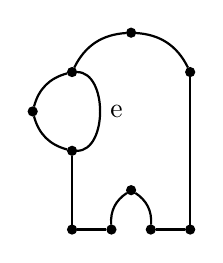
\begin{tikzpicture}[node distance={10mm}, thick, main/.style = {draw,circle,fill,inner sep=1pt}] 
  \node[main] (1) at (0,0) {}; 
  \node[main] (3) at (-0.5,0.5) {}; 
  \node[main] (4) at (0, 1) {}; 
  \node[main] (5) at (0, -1) {}; 
  \node[main] (6) at (1.5, -1) {}; 
  \node[main] (7) at (0.75, 1.5) {}; 
  \node[main] (8) at (1.5, 1) {}; 
  \node[main] (9) at (0.5, -1) {}; 
  \node[main] (10) at (1, -1) {}; 
  \node[main] (11) at (0.75, -0.5) {}; 
  \draw (1) to [bend left] (3);
  \draw (1) to [bend right=90]
node[midway, right] {e} (4) ;
  \draw (3) to [bend left] (4);
  \draw (4) to [bend left] (7);
  \draw (7) to [bend left] (8);
  \draw (8) to (6);
  \draw (5) to (9);
  \draw (6) to (10);
  \draw (9) to [bend left] (11);
  \draw (10) to [bend right] (11);
  \draw (5) to (1);
\end{tikzpicture} 
\end{subfigure}
\begin{subfigure}[h]{0.245\textwidth}
  \caption{$C _1$}
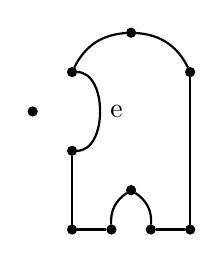
\begin{tikzpicture}[node distance={10mm}, thick, main/.style = {draw,circle,fill,inner sep=1pt}] 
  \node[main] (1) at (0,0) {}; 
  \node[main] (3) at (-0.5,0.5) {}; 
  \node[main] (4) at (0, 1) {}; 
  \node[main] (5) at (0, -1) {}; 
  \node[main] (6) at (1.5, -1) {}; 
  \node[main] (7) at (0.75, 1.5) {}; 
  \node[main] (8) at (1.5, 1) {}; 
  \node[main] (9) at (0.5, -1) {}; 
  \node[main] (10) at (1, -1) {}; 
  \node[main] (11) at (0.75, -0.5) {}; 
  \draw (1) to [bend right=90]
node[midway, right] {e} (4) ;
  \draw (4) to [bend left] (7);
  \draw (7) to [bend left] (8);
  \draw (8) to (6);
  \draw (5) to (9);
  \draw (6) to (10);
  \draw (9) to [bend left] (11);
  \draw (10) to [bend right] (11);
  \draw (5) to (1);
\end{tikzpicture} 
\end{subfigure}
\begin{subfigure}[h]{0.245\textwidth}
  \caption{$C _2$}
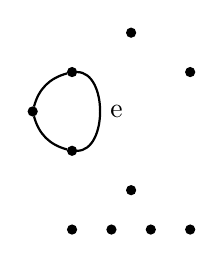
\begin{tikzpicture}[node distance={10mm}, thick, main/.style = {draw,circle,fill,inner sep=1pt}] 
  \node[main] (1) at (0,0) {}; 
  \node[main] (3) at (-0.5,0.5) {}; 
  \node[main] (4) at (0, 1) {}; 
  \node[main] (5) at (0, -1) {}; 
  \node[main] (6) at (1.5, -1) {}; 
  \node[main] (7) at (0.75, 1.5) {}; 
  \node[main] (8) at (1.5, 1) {}; 
  \node[main] (9) at (0.5, -1) {}; 
  \node[main] (10) at (1, -1) {}; 
  \node[main] (11) at (0.75, -0.5) {}; 
  \draw (1) to [bend left] (3);
  \draw (1) to [bend right=90]
node[midway, right] {e} (4) ;
  \draw (3) to [bend left] (4);
\end{tikzpicture} 
\end{subfigure}
\begin{subfigure}[h]{0.245\textwidth}
  \caption{$C _3$} 
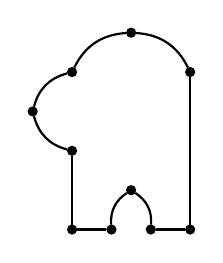
\begin{tikzpicture}[node distance={10mm}, thick, main/.style = {draw,circle,fill,inner sep=1pt}] 
  \node[main] (1) at (0,0) {}; 
  \node[main] (3) at (-0.5,0.5) {}; 
  \node[main] (4) at (0, 1) {}; 
  \node[main] (5) at (0, -1) {}; 
  \node[main] (6) at (1.5, -1) {}; 
  \node[main] (7) at (0.75, 1.5) {}; 
  \node[main] (8) at (1.5, 1) {}; 
  \node[main] (9) at (0.5, -1) {}; 
  \node[main] (10) at (1, -1) {}; 
  \node[main] (11) at (0.75, -0.5) {}; 
  \draw (1) to [bend left] (3);
  \draw (3) to [bend left] (4);
  \draw (4) to [bend left] (7);
  \draw (7) to [bend left] (8);
  \draw (8) to (6);
  \draw (5) to (9);
  \draw (6) to (10);
  \draw (9) to [bend left] (11);
  \draw (10) to [bend right] (11);
  \draw (5) to (1);
\end{tikzpicture} 
\end{subfigure}
                  \end{figure}

% We can say that a set $X \subseteq E$ is independent if and only if, it does not contain any circuit.
% The concept of circuits points towards something similar to a complement of the independent sets, but not completely. It is only the minimal dependent, and not all dependet subsets. We now have the following theorem.

\begin{lemma}\label{lem:circuits-have-properties}
  All circuits in a matroid satisfy (C1), (C2) and (C3).
\end{lemma}

\begin{proof} We will prove each property individually:
  
\begin{enumerate}
    \item[(C1)] $\emptyset \in \mathcal I$, therefore $\emptyset$ is not dependent (which means it cannot be a circuit)
    \item[(C2)] A counterexample to this clause would violate $C _2$ being minimal.
    \item[(C3)] Assume a counterexample exists. Because $C _1 \cup C _2 - e$ does not contain a circuit, it must be an element of $\mathcal I$. 

        We claim that $C _2 \setminus C _1$ is nonempty. Assume this is not the case. That would imply $C _2 \subseteq C _1$, but $C _1 \neq C _2 $ by (C3), which means that $C _1 $ is a proper subset of $C _2$. As both $C _1 $ and $C _2 $ are members of $\mathcal C$, this violates (C2), and is a contradiction. We can then assume some $f \in C _2 \setminus C _1 $ exists.

        As $C _2$ is minimally dependent, we know that $C _2 - f$ is independent. Let $I$ be a maximal independent subset of $C _2 \cup C _1$ which is a superset of $C _2 - f$. Clearly, $f \not\in I$ (otherwise $C _2 \subseteq I \in \mathcal I$). Furthermore, as $C _1 $ is a circuit, we know that $C _1 \not \subseteq I \in \mathcal I$ (otherwise $C _1$ would be independent). This means some $g \in C _1$ exists such that $g \not\in I$. As $f \in C _2  \setminus  C _2$, we know that $f \neq g$.

        As $I \subseteq C _1 \cup C _2$ and $f, g \in C _1 \cup C _2$ but $f, g \not\in I$, we can infer that 
        \begin{align*}
        |I| \leq |C _1 \cup C _2 - f - g| = |C _1 \cup C _2| - 2.
        \end{align*}

        We also notice that $|C _1 \cup C _2 - e| = |C _1 \cup C _2 | - 1$. We can now conclude by transitivity with $|C _1 \cup C _2 | - 2 < |C _1 \cup C _2 | - 1$ that $|I| < |C _1 \cup C _2 - e|$. We recall that both $I$ and $C _1 \cup C _2 - e$ are members of $\mathcal I$. We can apply (I3) to generate a superset of $I$ which contradicts it's maximality.
\end{enumerate}
\end{proof}

\begin{theorem}\label{thm:matroid-circuit-definition}
Let $E$ be a set and $\mathcal C$ be a collection of subsets of $E$ which satisfies the conditions outlined above. Let  $\mathcal I$  be the collection of subsets of $E$ that contain no member of $\mathcal C$, that is 

\begin{align}
   % \forall X \in \mathcal{I}, \forall C \in \mathcal C,  C \not \subseteq X. 
   \mathcal{I} = \{I \in 2^E |\; \text{for all } \; C \in \mathcal{C}\; \text{we have} \; C \not\subseteq I\}
    \label{independent-sets-from-circuits}
\end{align}

    The pair $(E,\mathcal I)$ is a matroid having $\mathcal C$ as its collection of circuits.
\end{theorem}

\begin{proof} We start by showing that $\mathcal I $ satisfies the necessary conditions for $(E, \mathcal I )$ to be a matroid:
    \begin{enumerate} 
        \item[(I1)] The only subset of $\emptyset $ is $ \emptyset $, but $ \emptyset \not\in \mathcal C $, so $ \emptyset $ satisfies (\ref{independent-sets-from-circuits}), hence $\emptyset \in \mathcal I$.
        \item[(I2)] Assume we have $X \subseteq Y \in \mathcal I$. Assume that $X \not\in I$, i.e.\ there exists some $C \in \mathcal C $ such that $C \subseteq X$. We recall that $\subseteq $ is transitive, thus $C \subseteq Y$ and $Y \not\in I$, hence a contradiction.
        \item[(I3)] Given $X, Y \in \mathcal I $ with $|X| < |Y|$ we must show there exists some $e \in Y \setminus X$ such that $X \cup \{e\} \in \mathcal I$. Assume that such an $e$ does not exist, i.e.\ for all $e \in Y \setminus X$ we have some circuit $C _e \in \mathcal C $ such that $C _e \subseteq X \cup \{e\}$. We obviously have $e \in C_e$, because otherwise $C_e \subseteq X$ and $X \not\in \mathcal I$.


     Let $X' = X \setminus Y$ and $Y' = Y \setminus X$. We will prove the statement by induction: given some set $S \subseteq X'$, a set of circuits $D \subseteq \mathcal C$ with $\forall C \in D, C \subseteq  S \cup Y$ and a surjective but not injective function $f : D \to S$ such that $f(D)$ is maximal in size and $\forall C \in D, f(C) \in C$, our statement is proven. We will use induction on the size of $S$:
    \begin{enumerate}
      \item If $S = \{e\}$ only has one element, we know that $f$ is not injective, so we must have distinct $C _1, C _2 \in D$ such that $e = f(C _1 ) = f(C _2)$. We can use the $3$-rd circuit axiom to generate some circuit $C _3 \subseteq C _1 \cup C _2 - e$. We recall that $C _1 , C _2 \subseteq S \cup Y $, so $C _3 \subseteq S \cup Y - e$ which implies $C _3 \subseteq Y$, which is a contradiction.
        \item Inductive step. Assuming the statement is true for all choices of $S$ with $k$ elements, we will attempt to prove it is also true when $S$ has $k + 1$ elements. Recalling that $f$ is not injective, we must have distinct $C _1, C _2 \in D$ such that $f(C _1 ) = f(C _2)$. Let $g = f(C _1)$. We have $g \in C _1, C _2$, so by the $3$-rd circuit axiom we must have some circuit $C  _3 \subseteq C _1 \cup C _2 - g$. Let $S' = C _3 \cap X'$. 

            For all $e \in S'$, we claim there must exist some $C_e \in D$ such that $e = f(C_e)$. Assume this is not the case, i.e.\ there is some $e \in S'$ such that no valid choice of $C_e$ exists. Given that $e \in S'$, we know that either $e \in C_1$ or $e \in C_2$. After a potential swap, we assume that $e \in C_1$. We can now define $f'(C) = e$ when $C = C_1$ and $f'(C) = f(C)$. Because no choice of $C_e$ exists, we know that $e \not\in f(D)$. Because $f(C _1 ) = f(C _2 )$ we have $f(D) = f(D - C _1 )$ which lets us compute $f'(D) = f(D) \cup \{e\}$, which means $f(D)$ was not maximal, hence a contradiction. Our claim is then true.

            Define $D' = \{C_e | e \in S'\} \cup \{C _3 \}$. We've essentially proven in the last paragraph that $f : \{C_e | e \in S'\} \to S'$ is still a  surjective function. It then follows that $h = f : D' \to S'$ is surjective as well. By the Pigeonhole principle, we know $h$ cannot be injective, because $|D'| = |S'| + 1$. We are now almost ready to apply the induction hypothesis to $(S', D', h)$. We've shown a choice for $h$ exist. If this choice is not maximal, swap it with a maximal choice (we had to show that at least one choice exists for a maximal choice to exist). We can now apply the induction hypothesis, proving the statement.
    \end{enumerate}

    We notice that $X$ can be partitioned into $X'$ and $X \cap Y$, hence $|X| = |X'| + |X \cap Y|$. We can follow a similar process for $Y$. Combining the two together with the fact that $|X| < |Y|$ yields that $|X'| < |Y'|$. We know that $Y \in \mathcal I$ so $\forall e \in Y', C_e \not \subseteq  Y$, but $C_e \subseteq  X \cup \{e\}$ therefore there must exist some $c_e \in C_e \cap X'$. 

    We define $D = \{C_e, e \in Y'\}$, $f(C_e) = c_e$ and $S = f(D)$. Furthermore, we know that $f$ is not injective by the Pigeonhole principle (we have $|D| = |Y'| > |X'| \geq |S|$). We also know, by the definition of $S$, that $f$ is surjective. We've shown a choice of $f$ exists. If it is not maximal, swap it with a maximal choice. We can now apply the statement proven by induction to finish the proof.
\end{enumerate}


We now show that $C$ is a circuit for the newly defined matroid if and only if it is a member of $\mathcal C$. 
\begin{enumerate}
  \item[$\implies$]
  If $C$ is a circuit, then $C \not\in \mathcal I$, which means that $C$ contains some $D \in \mathcal C$. As $C$ is minimally dependent, all its proper subsets are independent, but members of $\mathcal C$ cannot be independent (as seen in the definition of $\mathcal I$), which implies that $C = D$, hence $C \in \mathcal C$.
  \item[$\impliedby$]
  Let $C \in \mathcal C$. Assume $C$ is not a circuit. Clearly, $C \not\in \mathcal I$ is implied by the definition of $\mathcal I$ seen above. This implies that $C$ is dependent but not a circuit, which means $C$ is not miminal. 

  A proper subset $D  \subseteqneq C$ must then exist such that $D$ is a circuit. We've already shown in the $\implies$ direction how this implies $D \in \mathcal C$. We have now constructed a contradiction to (C2), hence our assumption that such a circuit exists is false.

\end{enumerate}



  We can now conclude that $(E, \mathcal I)$ is indeed a matroid with $\mathcal C$ as it's set of circuits.
\end{proof}

\section{Graphic matroids}

TRYING TO DO GRAPHS, DONT LAUGH! (DO NOT TOUCH!)

First, we do not define graphs in completely the same way as in the graph theory class. We used the definition that a graph $G$ is an ordered pair $G = (V, E)$ where $V$ is a finite set (of vertices) and $E$ is a collection of two-element subsets of $V$ (of edges). We will extend the notion of edge to include \textit{loops} and \textit{parallel edges}. For this, we will first illustrate the two notions. Intuitively a loop is an edge going from a vertex to itself, one can also have multiple loops on a single vertex.


For example, in the figure \ref{ilustratinloops}, we have a vertex $a$ with a single loop and vertex $d$ with 3 loops.

\begin{figure}[H]
    \centering
    \subfloat[\centering Loops]{
    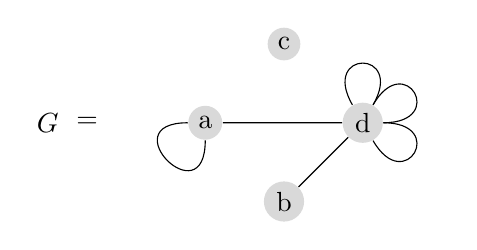
\begin{tikzpicture}[every loop/.style={}]

  \tikzstyle{vertex}=[circle,fill=black!15,minimum size=8pt,inner sep=2pt]

  \node (name) at (-2,0) {$G $};
  \node (another name) at (-1.5,0) {$ =$};
   
  
  \node[vertex] (v2) at (0,0)   {a};
  \node[vertex] (v3) at (1,-1)  {b};
  \node[vertex] (v4) at (1,1)  {c};
  \node[vertex] (v5) at (2,0)  {d};
  \draw (v2) edge[in=270,out=180, loop] node[below] {} ();

  \draw (v5) edge[in=300,out=0, loop] node[below] {} ();
  \draw (v5) edge[in=0,out=60, loop] node[below] {} ();
  \draw (v5) edge[in=60,out=120, loop] node[below] {} ();

  \draw (v2) -- (v5) -- (v3) -- cycle;

  
  %\draw[step=1cm,gray,very thin] (-2,-2) grid (4,4);

%\draw (v1) edge[in=270,out=180, loop] node[below] {2} ();

 
  
\end{tikzpicture}
    
    
    }%
    \qquad
    \subfloat[\centering Parallel edges]{
    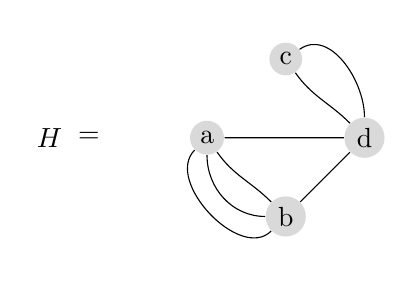
\begin{tikzpicture}[every loop/.style={}]

  \tikzstyle{vertex}=[circle,fill=black!15,minimum size=8pt,inner sep=2pt]

  \node (name) at (-2,0) {$H $};
  \node (another name) at (-1.5,0) {$ =$};
   
  
  \node[vertex] (v2) at (0,0)   {a};
  \node[vertex] (v3) at (1,-1)  {b};
  \node[vertex] (v4) at (1,1)  {c};
  \node[vertex] (v5) at (2,0)  {d};
  
  \draw (v2) edge[in=225,out=225] node[below] {} (v3);
  \draw (v2) edge[in=180,out=270] node[below] {} (v3);
  \draw (v2) edge[in=135,out=305] node[below] {} (v3);

  \draw (v4) edge[in=135,out=305] node[below] {} (v5);
  \draw (v4) edge[in=90,out=35] node[below] {} (v5);


  \draw (v2) -- (v5) -- (v3) -- cycle;

  
  %\draw[step=1cm,gray,very thin] (-2,-2) grid (4,4);

%\draw (v1) edge[in=270,out=180, loop] node[below] {2} ();

 
  
\end{tikzpicture}
    }%
    \caption{Graph $G$ with loops and graph $H$ with parallel edges}%
    \label{ilustratinloops}%
\end{figure}


Above we see graphs $G$ and $H$, one has loops and the other has parallel edges. One way to formalize both constructions, as done in \cite{oxley1} (for them to behave in the way we would like them to behave) is to define a graph to be an ordered pair $(V, E)$, where $V$ is a finite set, so unchanged, however $E$ is a \textit{multiset} of edges. This allows the same two-element subset of $V$ to appear multiple (but at most finitely many) times in $E$, even though it is the same set. Hence, we get parallel edges. For loops, we can get to a multiset consisting of a single element twice, and we also allow it to appear multiple times...
However, the formal construction is not so important, as we will see in the future and one can usually restrict to simple graphs, which are by our terminology the ones without loops or parallel edges. However, we are interested in \textit{properties} loops and parallel edges have. In particular, we see that by our definition of a cycle (a path (a walk (a sequence of adjacent vertices) which does not repeat vertices) which can repeat only one vertex (the ending and the starting vertex)), we have that if a loop is in a cycle, then the whole cycle consists only of that loop - we have one vertex appearing multiple times in a sequence - the beginning/ending vertex. Also, for parallel edges, at most one from a class of parallel edges connecting the same two vertices can appear in a cycle.


\begin{figure}[H]
\centering

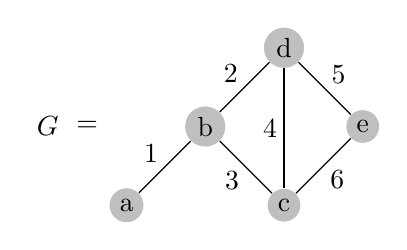
\begin{tikzpicture}[every loop/.style={}]

      \tikzstyle{vertex}=[circle,fill=black!25,minimum size=6pt,inner sep=2pt]

  \node (name) at (-2,0) {$G $};
  \node (another name) at (-1.5,0) {$ =$};
   
  \node[vertex] (v1) at (-1,-1) {a};
  \node[vertex] (v2) at (0,0)   {b};
  \node[vertex] (v3) at (1,-1)  {c};
  \node[vertex] (v4) at (1,1)  {d};
  \node[vertex] (v5) at (2,0)  {e};
  \draw (v1) -- node[midway, xshift=-0.5em, yshift=0.5em]{1} (v2) -- node[midway, xshift=-0.5em, yshift=-0.5em]{3} (v3) -- cycle;
  \draw (v2) -- node[midway, xshift=-0.5em, yshift=0.5em]{2} (v4) -- node[midway, xshift=0.5em, yshift=0.5em]{5} (v5) -- node[midway, xshift=0.5em, yshift=-0.5em]{6} (v3) -- cycle;
  \draw (v4) -- node[midway, xshift=-0.5em, yshift=0em]{4} (v3);

  
  %\draw[step=1cm,gray,very thin] (-2,-2) grid (4,4);

%\draw (v1) edge[in=270,out=180, loop] node[below] {2} ();

 
  
\end{tikzpicture}
\caption{Simple graph on 6 edges}
  \label{simp}

\end{figure}

Consider a concrete example of a simple graph and build a matroid out of it. Let us label the set of edges $E = \{1, 2, 3, \cdots, 6\}$. We will define a collection of subsets $\mathcal{C}$ of $E$ where $C \in \mathcal{C}$ if and only if the set of edges of $C$ forms a cycle in $G$. We check that 

    $$\mathcal{C} = \{\{2,3,4\}, \{4,5,6\}, \{2, 3, 5, 6\}\}.$$

Not surprisingly, the set $E$ with the collection $\mathcal{C}$ being as its set of circuits is, in fact, a matroid, we can check that there is no $\emptyset$ in $\mathcal{C}$, none of its members is properly contained in each other, and finally "circuit elimination axiom" works for all three possibilities of taking pairs of elements of $\mathcal{C}$. We will now prove that this works for a general graph.

\begin{theorem}
Let $G = (V, E)$ be a graph and let $C_1$, $C_2$ be sets of edges of two distinct cycles with a nonempty intersection. Then for any $e \in C_1 \cap C_2$ there exists a cycle $C_3 \subset C_1 \cup C_2 -e$, making the set $E$ of edges into a matroid with the set of circuits equal to the collection of cycles.
\end{theorem}

\begin{proof}

Let the cycle $C_1$ correspond to the sequence of incident vertices  $v_0, \cdots, v_n = v_0$ and let without loss of generality the special edge in the interesection be the edge $e = \{v_0, v_1\}$. Our goal is to find a cycle in the set of edges $C_1 \cup C_2 -e$, which is not difficult, the idea is that we go around $C_1$ until we can jump to $C_2$ for the first time, then we go back to $e$ via $C_2$ from the "backward direction".

Let $k$ be the smallest integer $1<k\leq n$ such that the vertex $v_k$ is in the cycle $C_2$. We know that such an integer exists because $v_n$ is in the cycle $C_2$. 

Let $v_k, w_{k+1}, w_{k+2}, \cdots, v_1$ be the path of vertices in the cycle $C_2$ which does not include the edge $e$. We know that such a path exists, because $C_2$ is a cycle, so from any two distinct vertices, in particular $v_k$ and $v_1$ there are two paths going from $v_k$ to $v_1$ including only the vertices of $C_2$ - we pick the one that does not include the edge $e$.

We claim that the cycle consisting of vertices $v_1, v_2, \cdots v_k, w_{k+1}, \cdots , v_1$ is the desired one and denote its set of edges by $C_3$. By construction the sequence of vertices $v_1, v_2, \cdots v_k, w_{k+1}, \cdots , v_1$ is a cycle, namely the neighboring vertices are incident and except $v_1$ there is no vertex repeating, because we have chosen $v_2, v_3, \cdots v_{k-1}$ to be disjoint from $C_2$. Crucially, $e \notin C_3$ because we have chosen path $v_k, w_{k+1}, \cdots v_1$ to not include the edge $e$ and $v_1, v_2, \cdots v_k$ does not include it because $e = \{v_n = v_0, v_1\}$ and there is no $v_0$ in our cycle. Finally, all of the vertices of $C_3$ are inside the vertices of $C_1$ and $C_2$ by construction so, to conclude the set $C_3$ has the desired property $C_3 \subset (C_1 \cup C_2) - e$.

We have to check to check the possibility that $e$ might be a loop or a parallel edge as well, the above argument works assuming $G$ is a simple graph. If $e$ is a parallel edge than the above argument does still hold since we only now that there is more than one edge between $v_0$
and $v_1$ which does not change anything. However, if $e$ is a loop then by our convention, a cycle consisting of a loop can just be that loop and nothing else, heuristically, because it begins and ends at a single vertex. So $C_1 = C_2 = \{e\}$ which is a contradiction, since we have assumed $C_1$ and $C_2$ are distinct.

To show that the set $E$ is a matroid with the collection $\mathcal{C}$ of cycles as circuits we only have to verify the first two circuit axioms. The empty set is by our defintion not a cycle, because by our defintion a cycle always includes a nonempty set of vertices it is build upon. If there are at least two vertices, than we have incident edges inside, and the only cycle on one vertex is a loop, which is still an edge.

The show the first property suppose we have two sets of edges of cycles such that $C_1 \subset C_2$ and assume for contradiction there is some $e \in C_2 - C_1$. Then (we are assuming neither of the cycles are loops, that case is obvious) the set of edges $C_2 - e$ corresponds to a path from the vertices which $e$ connects. However there is a cycle $C_1 \subset C_2 -e$ which is a subset of a path - a contradiction. So if $C_1 \subset C_2$ then $C_2 - C_1$ is empty, in particular then $C_2 = C1$ and all three circuit axioms are satisfied.



\end{proof}

\begin{defn}
    We call a matroid $M$ graphic it is isomporphic to $(E, \mathcal{I})$ where $E$ is the set of edges of some graph and the set of circuits is given by the set of all edge cycles.
\end{defn}

We thus know that given any graph $G$ we have natural matroid structure on its set of edges, by declaring graph cycles to be circuits. Because we know other equivalent descriptions of matroids it is natural to ask what are the independent sets or bases in the case of graphic matroids. 

Suppose that the set of edges $B$ is a base of a graphic matroid. We know that this means that $B$ is independent (interpretation of which in the case of graphic matroids we do not yet know) however, adding any element of $E-B$ to $B$, i.e. any edge not in $B$ to $B$, we get a \textit{dependent set}, which means it contains a circuit. By our defintion this means that it has to contain an edge cycle. Combining all we see that the set of edges $B$ has the property that it does not contain any cycles, however adding any edge makes a cycle - this is the precisely one of the equivalent characterizations of \textit{spanning forrests} - we cannot say spanning trees because the graph might not be connencted. 

Any independent set is a subset of some basis, so in graphic matroids the set of edges that is independent has to be a subset of some spanning forrest, which means it is just a forrest.

As an example we will show that many matroids shown until now are, in fact, graphic. 


 
\begin{figure}[H]
    \centering
    \subfloat[\centering Matrix $A$]{

    $$A = \begin{pmatrix}
        
        2 & 0 & 2 & 0 \\
        1 & -1 & 0 & 0 \\
        0 & 3 & 3 & 0
        
        
        \end{pmatrix}$$
        
    
    
    }
    \qquad
    \subfloat[\centering Graph $H$]{
    \begin{tikzpicture}[every loop/.style={}]

  \tikzstyle{vertex}=[circle,fill=black!15,minimum size=8pt,inner sep=2pt]

  \node (name) at (-2,-1.5) {$H $};
  \node (another name) at (-1.5,-1.5) {$ =$};
   
  
  \node[vertex] (v2) at (-1,-2)   {};
  \node[vertex] (v3) at (1,-2)  {};
 
  \node[vertex] (v5) at (0,-1)  {};
  

  \draw (v2) -- node[midway, xshift=0em, yshift=-0.5em]{1} (v3)  -- node[midway, xshift=0.6em, yshift=em]{2} (v5) -- node[midway, xshift=-0.6em, yshift=0em]{3} (v2)  --cycle;
  
  \draw (v5) edge[in=150,out=30, loop] node[above] {4} ();
  
  %\draw[step=1cm,gray,very thin] (-2,-2) grid (4,4);

%\draw (v1) edge[in=270,out=180, loop] node[below] {2} ();

 
  
\end{tikzpicture}
    }%
    \caption{Matroid $M[A]$ is graphic; it is isomprphic to the graphic matroid $G$}%
    \label{graphic}%
\end{figure}

In \ref{graphic} we see that the graph $H$ exactly to corresponds to the vector matroid formed on matrix $A$. Edge 4 is a loop, so a dependent set, corresponding to the fact that the fourth column is a zero vector. Similarly, any two element sets of nonzero vector are independent, corresponding to the fact that any two non-loop edges do not form a cycle in the graph. Finally, any set of three or more edges in dependent, which is easily seen in the graph because we have 3 vertices so the size of a spanning forrest is at most 3 - 1 = 2.




\section{Rank Function}

The rank function is a function $r:2^E \rightarrow \mathbb{Z}_{\geq0}$ that, when given a $X\subseteq E(M)$, gives you the cardinality of the maximal independent set contained in $X$. In other words:
$$ r(X) = \max\{\, |I| : I\in\mathcal{I} \text{ and } I\subseteq X \} $$
For example, $r(M):=r(E(M))=|B|$ for some $B\in\mathcal{B}(M)$. Like all the previous times, we can characterize the rank function with the following properties:

\begin{defn}
    Let $E$ be a non-empty finite set, and let $\rank : 2^E \rightarrow \mathbb{Z}_{\geq0}$ be a function satisfying:
    \begin{enumerate}
        \item[(R1)] If $X\subseteq E$, then $0 \leq \rank(X) \leq |X| $
        \item[(R2)] If $X\subseteq Y\subseteq E$, then $\rank(X)\leq\rank(Y)$
        \item[(R3)] If $X,Y\subseteq E$, then $\rank(X\cup Y)+\rank(X\cap Y) \leq \rank(X)+\rank(Y) $
    \end{enumerate}
\end{defn}

Below, we again find our example matroid drawing. This time, instead of using a new color, we will denote the rank of each set by writing it in subscript below the set. We can see that the rank of any set is at most its cardinality, and each subset of some set has at most the rank of that set. As always, it takes a bit more effort to show that the last property holds for a given matroid.

\begin{center}
\begin{tikzpicture}

\matrix (a) [matrix of math nodes, column sep=0.6cm, row sep=0.6cm,]{
 & & &\textcolor{cyan}{
1234}_2 & & & &\\
 \textcolor{cyan}{
123}_2& &\textcolor{cyan}{
124}_2 & &\textcolor{cyan}{
134}_1 &  & \textcolor{cyan}{
234}_2  \\
\textcolor{red}{12}_2 & \textcolor{blue}{13}_1 & \textcolor{cyan}{14}_1 & & \textcolor{red}{23}_2 & \textcolor{cyan}{
24}_1 & \textcolor{cyan}{
34}_1 \\
\textcolor{orange}{1}_1& &\textcolor{orange}{2}_1 & & \textcolor{orange}{3}_1& & \textcolor{blue}{4}_0 \\
& & & \textcolor{orange}{\emptyset}_0 &  & & \\
&&&&&& \\};

\foreach \i/\j in {1-4/2-1, 1-4/2-3, 1-4/2-5, 1-4/2-7, 2-1/3-1, 2-1/3-2, 2-1/3-5, 2-3/3-1, 2-3/3-3, 2-3/3-6, 2-5/3-2, 2-5/3-3, 2-5/3-7, 2-7/3-5, 2-7/3-6, 2-7/3-7, 3-1/4-1, 3-1/4-3, 3-2/4-1, 3-2/4-5, 3-3/4-1, 3-3/4-7, 3-5/4-3, 3-5/4-5, 3-6/4-3, 3-6/4-7, 3-7/4-7, 3-7/4-5, 4-1/5-4, 4-3/5-4, 4-5/5-4, 4-7/5-4}
\draw[double, line width = 0.005mm, color = brown] (a-\i) -- (a-\j);

\node[draw] at (0, -2.5){\small \textcolor{orange}{Independent set}, \textcolor{red}{Basis}, \textcolor{cyan}{Dependent set}, \textcolor{blue}{Circuit}, $\text{Set}_{\rank(\text{Set})}$ };

\end{tikzpicture}
\end{center}

Now, let us prove that the rank function of a matroid satisfy these properties:

\begin{proof}
    \,
    \begin{enumerate}
        \item Since the co-domain is $\mathbb{Z}_{\geq0}$, $0\leq\rank(X)$. Since the maximal independent set contained in $X$ is... contained in $X$, the cardinality of that set must be smaller or equal to $|X|$. Thus, $0\leq\rank(X)\leq|X|$.
        \item Let $I_X$ be a minimal independent set contained in $X$, so $\rank(X)=|I_X|$. $I_X\subseteq X\subseteq Y$ implies that $I_X$ is an independent set contained in $Y$. Since $I_X$ may or may not be a maximal independent set contained in $Y$, $\rank(X)=|I_X|\leq\rank(Y)$. 
        \item We assume that $A\subseteq B\subseteq E$. Let $I_{A\cap B}$ be a maximal independent set contained in $A\cap B$. Since $A\cap B\subseteq A\cup B$, $I_{A\cap B}$ must be an independent set contained in $A\cup B$. Let $I_{A\cup B}$ be $I_{A\cap B}$ extended to be a \textbf{maximal} independent set contained in $A\cup B$. 
        
        Now, et us take a look at $I_{A\cup B}\cap A$. Since the set is contained in $A$, (I2) tells us that $I_{A\cup B}\cap A$ is in independent set contained in $A$. Since the set may or may not be maximal in that regard, $|I_{A\cup B}\cap A|\leq \rank(A)$. Similarly, $|I_{A\cup B}\cap B|\leq \rank(B) $.
        
        $$ \rank(X)+\rank(Y) \geq |I_{A\cup B}\cap A|+|I_{A\cup B}\cap B| $$
        $$ = |(I_{A\cup B}\cap A)\cup(I_{A\cup B}\cap B)|+|(I_{A\cup B}\cap A)\cap(I_{A\cup B}\cap B)| $$
        $$ = |I_{A\cup B}\cap (A\cup B)|+|I_{A\cup B}\cap (A\cap B)| $$

        Since $I_{A\cup B}\subseteq A\cup B$, $I_{A\cup B}\cap(A\cup B) = I_{A\cup B}$.

        Since $I_{A\cap B}\subseteq I_{A\cup B}$, $I_{A\cup B}\cap (A\cap B) \supset I_{A\cap B}\cap (A\cap B) = I_{A\cap B} $. Let $e\in I_{A\cup B}\cap (A\cap B)$. Aiming for contradiction, suppose $e\notin I_{A\cap B}$. Since $I_{A\cap B}\cup e \subseteq I_{A\cup B} $, $I_{A\cap B}\cup e$ must be an independent set contained in $A\cap B$. This contradicts the fact that $I_{A\cap B}$ is a maximal in that regard. Thus, $e\in I_{A\cap B}$. This proves that $I_{A\cup B}\cap(A\cap B)\subseteq I_{A\cap B} $, which implies equality between the two sets.

        Thus,

        $$ \rank(X)+\rank(Y) \geq |I_{A\cup B}|+|I_{A\cap B}| = \rank(A\cup B)+\rank(A\cap B) $$
    \end{enumerate}
\end{proof}
One might observe that the rank of an independent set is the cardinality of the set itself. This is because the largest independent set that is contained in this independent set is of course the independent set itself. With this property, we can define the set of independent sets with the three properties of the rank function.
\begin{theorem}
    Let $E$ be a finite set, and let $\rank : 2^E \rightarrow \mathbb{Z}_{\geq0}$ be a function satisfying (R1)-(R3). Let $\mathcal{I} = \{ I\subseteq E : \rank(I)=|I| \} $. Then $(E,\mathcal{I})$ is a matroid with $\rank$ as its rank function.
\end{theorem}
Before we prove this, let's prove this small theorem first:
\begin{theorem}
\label{rankextension}
    Let $E$ be a finite set and $\rank:2^E\rightarrow \mathbb{Z}_{\geq0}$ be a function satisfying (R2) and (R3). Let $X,Y\subseteq E$. Then if for all $y\in Y-X$, $\rank(X\cup y)=\rank(X)$, then $\rank(X\cup Y)=\rank(Y)$.
\end{theorem}
\begin{proof}
    We will prove that the statement holds with $Y-X = \{a_1,a_2,\dots,a_k\}$ holds for all integers $k$.
    \begin{enumerate}
        \item Base case: $k=1$

        If $\rank(X\cup a_1)=\rank(X)$, then $\rank(X\cup Y)=\rank(X\cup(Y-X))=\rank(X\cup a_1)=\rank(X)$.
        \item Induction Step: Assume the statement holds for $k=n$.
        \item Let $k=n+1$: Assume that $Y-X=\{a_1,\dots,a_{n+1}\}$ for all $i\in\{1,\dots,n+1\}$ $\rank(X\cup a_i)=\rank(X)$. Then, using the assumption and our induction assumption, 
        $$ \rank(X)+\rank(X) = \rank(X\cup \{a_1,\dots,a_n\})+\rank(X\cup a_{n+1}) $$
        Using (R3), we get
        $$ \geq \rank([X\cup\{a_1,\dots,a_n\}]\cup [X\cup a_{n+1}]) + \rank([X\cup\{a_1,\dots,a_n\}]\cap [X\cup a_{n+1}]) $$
        $$ = \rank(X\cup\{a_1,\dots,a_{n+1}\}) + \rank(X) $$
        Using (R2), we get
        $$ \geq \rank(X)+\rank(X) $$
        Since $\rank(X)+\rank(X)$ is on both sides, equality holds throughout. Thus, $\rank(X\cup\{a_1,\dots,a_{n+1}\})=\rank(X\cup Y)=\rank(X)$. And thus, the statement holds for $k=n+1$.
    \end{enumerate}
    Thus, by mathematical induction, the statement holds for all integers $k$.
\end{proof}
Finally, we can prove Theorem 5:
\begin{proof}
    To prove that $(E,\mathcal{I})$ is a matroid, we will check if $\mathcal{I}$ satisfies (I1)-(I3).
    \begin{enumerate}
        \item (R1) tells us that $0\leq\rank(\emptyset)\leq|\emptyset|=0$, which implies that $\rank(\emptyset)=0=|\emptyset|$, which means that $\emptyset\in\mathcal{I}$, so (I1) is satisfied.
        \item Assume we have $J\subseteq I\in\mathcal{I}$. Then, using (R3),
        $$ \rank(J)+\rank(I-J) \geq \rank(J\cup[I-J])+\rank(J\cap[I-J]) = \rank(I)+\rank(\emptyset)=|I| $$
        Using (R2), we also get that
        $$ \rank(J)+\rank(I-J) \leq |J|+\rank(I-J) \leq |J|+|I-J| = |I| $$
        This implies that equality must hold throughout. At last, we show that
        $$ \rank(J)+\rank(I-J) = |J|+\rank(I-J) \Rightarrow \rank(J)=|J| $$
        Thus, $J\in\mathcal{I}$, so {I2} is satisfied.
        
        \item Suppose (I3) does not hold for some $I,J\in\mathcal{I}$ with $|I|>|J|$. Then for all $e\in I-J$, $J\cup e\notin \mathcal{I}$. Also, remember that $I,J\in\mathcal{I}$ means that $\rank(I)=|I|$ and $\rank(J)=|J|$.

        Since $J\subseteq J\cup e$, we can use (R1) and (R2) to see that
        $$ |J|=\rank(J)\leq\rank(J\cup e)|\leq|J\cup e|=|J|+1 $$
        $J\cup e\notin \mathcal{I}$ tells us that $\rank(J\cup e)\neq|J\cup e|$, so that must mean that $\rank(J\cup e)$ is equal to what's on the left-hand side, so $\rank(J)$.

        This gives us that for all $e\in I-J$, $\rank(J\cup e)=\rank(J)$, which, according to Theorem 6, implies that $\rank(J\cup I)=\rank(J)=|J|$. However, since $I\subseteq J\cup I$, (R2) tells us that $\rank(J\cup I) \geq \rank(I) = |I|$, which means that $|J|\geq|I|$. This contradicts our assumption that $|J|<|I|$. Thus, (I3) is satisfied.
    \end{enumerate}
    Thus, $(E,\mathcal{I})$ is a matroid.
\end{proof}


\section{Graphic matroids}

TRYING TO DO GRAPHS, DONT LAUGH! (DO NOT TOUCH!)

First, we do not define graphs in completely the same way as in the graph theory class. We used the definition that a graph $G$ is an ordered pair $G = (V, E)$ where $V$ is a finite set (of vertices) and $E$ is a collection of two-element subsets of $V$ (of edges). We will extend the notion of edge to include \textit{loops} and \textit{parallel edges}. For this, we will first illustrate the two notions. Intuitively a loop is an edge going from a vertex to itself, one can also have multiple loops on a single vertex.


For example, in the figure \ref{ilustratinloops}, we have a vertex $a$ with a single loop and vertex $d$ with 3 loops.

\begin{figure}[H]
    \centering
    \subfloat[\centering Loops]{
    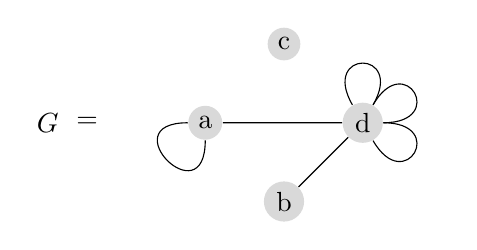
\begin{tikzpicture}[every loop/.style={}]

  \tikzstyle{vertex}=[circle,fill=black!15,minimum size=8pt,inner sep=2pt]

  \node (name) at (-2,0) {$G $};
  \node (another name) at (-1.5,0) {$ =$};
   
  
  \node[vertex] (v2) at (0,0)   {a};
  \node[vertex] (v3) at (1,-1)  {b};
  \node[vertex] (v4) at (1,1)  {c};
  \node[vertex] (v5) at (2,0)  {d};
  \draw (v2) edge[in=270,out=180, loop] node[below] {} ();

  \draw (v5) edge[in=300,out=0, loop] node[below] {} ();
  \draw (v5) edge[in=0,out=60, loop] node[below] {} ();
  \draw (v5) edge[in=60,out=120, loop] node[below] {} ();

  \draw (v2) -- (v5) -- (v3) -- cycle;

  
  %\draw[step=1cm,gray,very thin] (-2,-2) grid (4,4);

%\draw (v1) edge[in=270,out=180, loop] node[below] {2} ();

 
  
\end{tikzpicture}
    
    
    }%
    \qquad
    \subfloat[\centering Parallel edges]{
    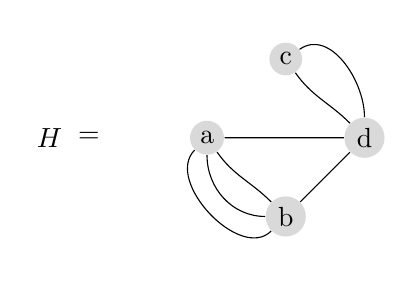
\begin{tikzpicture}[every loop/.style={}]

  \tikzstyle{vertex}=[circle,fill=black!15,minimum size=8pt,inner sep=2pt]

  \node (name) at (-2,0) {$H $};
  \node (another name) at (-1.5,0) {$ =$};
   
  
  \node[vertex] (v2) at (0,0)   {a};
  \node[vertex] (v3) at (1,-1)  {b};
  \node[vertex] (v4) at (1,1)  {c};
  \node[vertex] (v5) at (2,0)  {d};
  
  \draw (v2) edge[in=225,out=225] node[below] {} (v3);
  \draw (v2) edge[in=180,out=270] node[below] {} (v3);
  \draw (v2) edge[in=135,out=305] node[below] {} (v3);

  \draw (v4) edge[in=135,out=305] node[below] {} (v5);
  \draw (v4) edge[in=90,out=35] node[below] {} (v5);


  \draw (v2) -- (v5) -- (v3) -- cycle;

  
  %\draw[step=1cm,gray,very thin] (-2,-2) grid (4,4);

%\draw (v1) edge[in=270,out=180, loop] node[below] {2} ();

 
  
\end{tikzpicture}
    }%
    \caption{Graph $G$ with loops and graph $H$ with parallel edges}%
    \label{ilustratinloops}%
\end{figure}


Above we see graphs $G$ and $H$, one has loops and the other has parallel edges. One way to formalize both constructions, as done in \cite{oxley1} (for them to behave in the way we would like them to behave) is to define a graph to be an ordered pair $(V, E)$, where $V$ is a finite set, so unchanged, however $E$ is a \textit{multiset} of edges. This allows the same two-element subset of $V$ to appear multiple (but at most finitely many) times in $E$, even though it is the same set. Hence, we get parallel edges. For loops, we can get to a multiset consisting of a single element twice, and we also allow it to appear multiple times...
However, the formal construction is not so important, as we will see in the future and one can usually restrict to simple graphs, which are by our terminology the ones without loops or parallel edges. However, we are interested in \textit{properties} loops and parallel edges have. In particular, we see that by our definition of a cycle (a path (a walk (a sequence of adjacent vertices) which does not repeat vertices) which can repeat only one vertex (the ending and the starting vertex)), we have that if a loop is in a cycle, then the whole cycle consists only of that loop - we have one vertex appearing multiple times in a sequence - the beginning/ending vertex. Also, for parallel edges, at most one from a class of parallel edges connecting the same two vertices can appear in a cycle.


\begin{figure}[H]
\centering

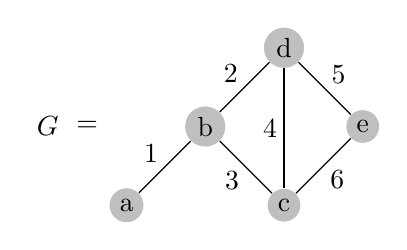
\begin{tikzpicture}[every loop/.style={}]

      \tikzstyle{vertex}=[circle,fill=black!25,minimum size=6pt,inner sep=2pt]

  \node (name) at (-2,0) {$G $};
  \node (another name) at (-1.5,0) {$ =$};
   
  \node[vertex] (v1) at (-1,-1) {a};
  \node[vertex] (v2) at (0,0)   {b};
  \node[vertex] (v3) at (1,-1)  {c};
  \node[vertex] (v4) at (1,1)  {d};
  \node[vertex] (v5) at (2,0)  {e};
  \draw (v1) -- node[midway, xshift=-0.5em, yshift=0.5em]{1} (v2) -- node[midway, xshift=-0.5em, yshift=-0.5em]{3} (v3) -- cycle;
  \draw (v2) -- node[midway, xshift=-0.5em, yshift=0.5em]{2} (v4) -- node[midway, xshift=0.5em, yshift=0.5em]{5} (v5) -- node[midway, xshift=0.5em, yshift=-0.5em]{6} (v3) -- cycle;
  \draw (v4) -- node[midway, xshift=-0.5em, yshift=0em]{4} (v3);

  
  %\draw[step=1cm,gray,very thin] (-2,-2) grid (4,4);

%\draw (v1) edge[in=270,out=180, loop] node[below] {2} ();

 
  
\end{tikzpicture}
\caption{Simple graph on 6 edges}
  \label{simp}

\end{figure}

Consider a concrete example of a simple graph and build a matroid out of it. Let us label the set of edges $E = \{1, 2, 3, \cdots, 6\}$. We will define a collection of subsets $\mathcal{C}$ of $E$ where $C \in \mathcal{C}$ if and only if the set of edges of $C$ forms a cycle in $G$. We check that 

    $$\mathcal{C} = \{\{2,3,4\}, \{4,5,6\}, \{2, 3, 5, 6\}\}.$$

Not surprisingly, the set $E$ with the collection $\mathcal{C}$ being as its set of circuits is, in fact, a matroid, we can check that there is no $\emptyset$ in $\mathcal{C}$, none of its members is properly contained in each other, and finally "circuit elimination axiom" works for all three possibilities of taking pairs of elements of $\mathcal{C}$. We will now prove that this works for a general graph.

\begin{theorem}
Let $G = (V, E)$ be a graph and let $C_1$, $C_2$ be sets of edges of two distinct cycles with a nonempty intersection. Then for any $e \in C_1 \cap C_2$ there exists a cycle $C_3 \subset C_1 \cup C_2 -e$, making the set $E$ of edges into a matroid with the set of circuits equal to the collection of cycles.
\end{theorem}

\begin{proof}

Let the cycle $C_1$ correspond to the sequence of incident vertices  $v_0, \cdots, v_n = v_0$ and let without loss of generality the special edge in the interesection be the edge $e = \{v_0, v_1\}$. Our goal is to find a cycle in the set of edges $C_1 \cup C_2 -e$, which is not difficult, the idea is that we go around $C_1$ until we can jump to $C_2$ for the first time, then we go back to $e$ via $C_2$ from the "backward direction".

Let $k$ be the smallest integer $1<k\leq n$ such that the vertex $v_k$ is in the cycle $C_2$. We know that such an integer exists because $v_n$ is in the cycle $C_2$. 

Let $v_k, w_{k+1}, w_{k+2}, \cdots, v_1$ be the path of vertices in the cycle $C_2$ which does not include the edge $e$. We know that such a path exists, because $C_2$ is a cycle, so from any two distinct vertices, in particular $v_k$ and $v_1$ there are two paths going from $v_k$ to $v_1$ including only the vertices of $C_2$ - we pick the one that does not include the edge $e$.

We claim that the cycle consisting of vertices $v_1, v_2, \cdots v_k, w_{k+1}, \cdots , v_1$ is the desired one and denote its set of edges by $C_3$. By construction the sequence of vertices $v_1, v_2, \cdots v_k, w_{k+1}, \cdots , v_1$ is a cycle, namely the neighboring vertices are incident and except $v_1$ there is no vertex repeating, because we have chosen $v_2, v_3, \cdots v_{k-1}$ to be disjoint from $C_2$. Crucially, $e \notin C_3$ because we have chosen path $v_k, w_{k+1}, \cdots v_1$ to not include the edge $e$ and $v_1, v_2, \cdots v_k$ does not include it because $e = \{v_n = v_0, v_1\}$ and there is no $v_0$ in our cycle. Finally, all of the vertices of $C_3$ are inside the vertices of $C_1$ and $C_2$ by construction so, to conclude the set $C_3$ has the desired property $C_3 \subset (C_1 \cup C_2) - e$.

We have to check to check the possibility that $e$ might be a loop or a parallel edge as well, the above argument works assuming $G$ is a simple graph. If $e$ is a parallel edge than the above argument does still hold since we only now that there is more than one edge between $v_0$
and $v_1$ which does not change anything. However, if $e$ is a loop then by our convention, a cycle consisting of a loop can just be that loop and nothing else, heuristically, because it begins and ends at a single vertex. So $C_1 = C_2 = \{e\}$ which is a contradiction, since we have assumed $C_1$ and $C_2$ are distinct.

To show that the set $E$ is a matroid with the collection $\mathcal{C}$ of cycles as circuits we only have to verify the first two circuit axioms. The empty set is by our defintion not a cycle, because by our defintion a cycle always includes a nonempty set of vertices it is build upon. If there are at least two vertices, than we have incident edges inside, and the only cycle on one vertex is a loop, which is still an edge.

The show the first property suppose we have two sets of edges of cycles such that $C_1 \subset C_2$ and assume for contradiction there is some $e \in C_2 - C_1$. Then (we are assuming neither of the cycles are loops, that case is obvious) the set of edges $C_2 - e$ corresponds to a path from the vertices which $e$ connects. However there is a cycle $C_1 \subset C_2 -e$ which is a subset of a path - a contradiction. So if $C_1 \subset C_2$ then $C_2 - C_1$ is empty, in particular then $C_2 = C1$ and all three circuit axioms are satisfied.



\end{proof}

\begin{defn}
    We call a matroid $M$ graphic it is isomporphic to $(E, \mathcal{I})$ where $E$ is the set of edges of some graph and the set of circuits is given by the set of all edge cycles.
\end{defn}

We thus know that given any graph $G$ we have natural matroid structure on its set of edges, by declaring graph cycles to be circuits. Because we know other equivalent descriptions of matroids it is natural to ask what are the independent sets or bases in the case of graphic matroids. 

Suppose that the set of edges $B$ is a base of a graphic matroid. We know that this means that $B$ is independent (interpretation of which in the case of graphic matroids we do not yet know) however, adding any element of $E-B$ to $B$, i.e. any edge not in $B$ to $B$, we get a \textit{dependent set}, which means it contains a circuit. By our defintion this means that it has to contain an edge cycle. Combining all we see that the set of edges $B$ has the property that it does not contain any cycles, however adding any edge makes a cycle - this is the precisely one of the equivalent characterizations of \textit{spanning forrests} - we cannot say spanning trees because the graph might not be connencted. 

Any independent set is a subset of some basis, so in graphic matroids the set of edges that is independent has to be a subset of some spanning forrest, which means it is just a forrest.

As an example we will show that many matroids shown until now are, in fact, graphic. 


 
\begin{figure}[H]
    \centering
    \subfloat[\centering Matrix $A$]{

    $$A = \begin{pmatrix}
        
        2 & 0 & 2 & 0 \\
        1 & -1 & 0 & 0 \\
        0 & 3 & 3 & 0
        
        
        \end{pmatrix}$$
        
    
    
    }
    \qquad
    \subfloat[\centering Graph $H$]{
    \begin{tikzpicture}[every loop/.style={}]

  \tikzstyle{vertex}=[circle,fill=black!15,minimum size=8pt,inner sep=2pt]

  \node (name) at (-2,-1.5) {$H $};
  \node (another name) at (-1.5,-1.5) {$ =$};
   
  
  \node[vertex] (v2) at (-1,-2)   {};
  \node[vertex] (v3) at (1,-2)  {};
 
  \node[vertex] (v5) at (0,-1)  {};
  

  \draw (v2) -- node[midway, xshift=0em, yshift=-0.5em]{1} (v3)  -- node[midway, xshift=0.6em, yshift=em]{2} (v5) -- node[midway, xshift=-0.6em, yshift=0em]{3} (v2)  --cycle;
  
  \draw (v5) edge[in=150,out=30, loop] node[above] {4} ();
  
  %\draw[step=1cm,gray,very thin] (-2,-2) grid (4,4);

%\draw (v1) edge[in=270,out=180, loop] node[below] {2} ();

 
  
\end{tikzpicture}
    }%
    \caption{Matroid $M[A]$ is graphic; it is isomprphic to the graphic matroid $G$}%
    \label{graphic}%
\end{figure}

In \ref{graphic} we see that the graph $H$ exactly to corresponds to the vector matroid formed on matrix $A$. Edge 4 is a loop, so a dependent set, corresponding to the fact that the fourth column is a zero vector. Similarly, any two element sets of nonzero vector are independent, corresponding to the fact that any two non-loop edges do not form a cycle in the graph. Finally, any set of three or more edges in dependent, which is easily seen in the graph because we have 3 vertices so the size of a spanning forrest is at most 3 - 1 = 2.




\newpage
\section{Rank Function}

The rank function is a function $\rank :2^E \rightarrow \mathbb{Z}_{\geq0}$ that, when given a $X\subseteq E(M)$, gives you the cardinality of a maximal independent set contained in $X$. In other words:

$$ \rank(X) = \max\{\, |I| \; | \,\, I\in\mathcal{I} \text{ and } I\subseteq X \} $$
For example, $\rank(E(M))=|B|$ for some $B\in\mathcal{B}(M)$, and we define $\rank(M) = \rank(E(M))$. We can characterize the rank function with the following properties:

\begin{theorem}
    Let $M$ be a matroid on a ground set $E$, and let $\rank : 2^E \rightarrow \mathbb{Z}_{\geq0}$ be its rank function. Then $\rank$ satisfies these properties.
    \begin{enumerate}
        \item[(R1)] If $X\subseteq E$, then $0 \leq \rank(X) \leq |X| $
        \item[(R2)] If $X\subseteq Y\subseteq E$, then $\rank(X)\leq\rank(Y)$
        \item[(R3)] If $X,Y\subseteq E$, then $\rank(X\cup Y)+\rank(X\cap Y) \leq \rank(X)+\rank(Y) $
    \end{enumerate}
\end{theorem}

In Figure \ref{fig:1234-matroid-rank}, we again find our example matroid drawing. We denote the rank of each set by writing it in subscript below the set. We can see that the rank of any set is at most its cardinality, and each subset of some set has at most the rank of that set. As always, it takes a bit more effort to show that the last property holds for a given matroid.

\begin{figure}[H]
    \begin{center}
    \begin{tikzpicture}
    
    \matrix (a) [matrix of math nodes, column sep=0.6cm, row sep=0.6cm,]{
     & & &\textcolor{cyan}{
    1234}_2 & & & &\\
     \textcolor{cyan}{
    123}_2& &\textcolor{cyan}{
    124}_2 & &\textcolor{cyan}{
    134}_1 &  & \textcolor{cyan}{
    234}_2  \\
    \textcolor{red}{12}_2 & \textcolor{blue}{13}_1 & \textcolor{cyan}{14}_1 & & \textcolor{red}{23}_2 & \textcolor{cyan}{
    24}_1 & \textcolor{cyan}{
    34}_1 \\
    \textcolor{orange}{1}_1& &\textcolor{orange}{2}_1 & & \textcolor{orange}{3}_1& & \textcolor{blue}{4}_0 \\
    & & & \textcolor{orange}{\emptyset}_0 &  & & \\
    &&&&&& \\};
    
    \foreach \i/\j in {1-4/2-1, 1-4/2-3, 1-4/2-5, 1-4/2-7, 2-1/3-1, 2-1/3-2, 2-1/3-5, 2-3/3-1, 2-3/3-3, 2-3/3-6, 2-5/3-2, 2-5/3-3, 2-5/3-7, 2-7/3-5, 2-7/3-6, 2-7/3-7, 3-1/4-1, 3-1/4-3, 3-2/4-1, 3-2/4-5, 3-3/4-1, 3-3/4-7, 3-5/4-3, 3-5/4-5, 3-6/4-3, 3-6/4-7, 3-7/4-7, 3-7/4-5, 4-1/5-4, 4-3/5-4, 4-5/5-4, 4-7/5-4}
    \draw[double, line width = 0.005mm, color = brown] (a-\i) -- (a-\j);
    
    \node[draw] at (0, -2.5){\small \textcolor{orange}{Independent set}, \textcolor{red}{Basis}, \textcolor{cyan}{Dependent set}, \textcolor{blue}{Circuit}, $\text{Set}_{\rank(\text{Set})}$ };
    \end{tikzpicture}
    \end{center}

    \caption{Description of a 4-element matroid, with the rank of each set as subscript.}
    \label{fig:1234-matroid-rank}
\end{figure}




Now, let us prove that the rank function of a matroid satisfies these properties. 

\begin{proof}
    \begin{enumerate}
        \item[(R1)] Since the co-domain of $\rank$ is $\mathbb{Z}_{\geq0}$ then  $\rank(X) \geq 0$. Let $I_X$ be a maximal independent set contained in $X$. By definition, we see that $|I_X|=\rank(X)$. Since $X\supseteq I_X$, it follows that $|X| \geq |I_X| = \rank(X)$.       Thus, $0\leq\rank(X)\leq|X|$ what we wanted to show.
        
        \item[(R2)] Let $I_X$ be a minimal independent set contained in $X$, so $\rank(X)=|I_X|$. $I_X\subseteq X\subseteq Y$ implies that $I_X$ is an independent set contained in $Y$. Since $I_X$ is an independent set contained in $Y$ then by definition $|I_X|\leq \rank(Y)$ since $\rank(Y)$ is the size of the \textit{largest} independent set contained in $Y$. Finally, we get that $\rank(X)=|I_X|\leq \rank(Y)$ what we wanted to show.
        
        \item[(R3)] We assume that $A\subseteq B\subseteq E$. Let $I_{A\cap B}$ be a maximal independent set contained in $A\cap B$. Since $A\cap B\subseteq A\cup B$, it means that $I_{A\cap B}$ must be an independent set contained in $A\cup B$. Let $I_{A\cup B}$ be $I_{A\cap B}$ \textit{extended} to be a \textbf{maximal} independent set contained in $A\cup B$. So $I_{A\cap B}\subseteq I_{A\cup B} \subseteq A\cup B$. 
        
        Now, let us take a look at the set $I_{A\cup B}\cap A$. Since the set is contained in $A$ and $I_{A\cup B}$, the property (I2) tells us that $I_{A\cup B}\cap A$ is in independent set contained in $A$. Since the set may or may not be maximal we know by definition, $|I_{A\cup B}\cap A|\leq \rank(A)$. Similarly, $|I_{A\cup B}\cap B|\leq \rank(B) $.

        We will now use the well known fact that for any sets $X$ and $Y$, it holds that $|X\cup Y|=|X|+|Y|-|X\cap Y|$, in other words $|X|+|Y|=|X\cup Y|+|X\cap Y|$.
        
        \begin{align*}
            \rank(A)+\rank(B) &\geq |I_{A\cup B}\cap A|+|I_{A\cup B}\cap B| 
            \\&=  |(I_{A\cup B}\cap A)\cup(I_{A\cup B}\cap B)|
             +|(I_{A\cup B}\cap A)\cap(I_{A\cup B}\cap B)| 
            \\&=  |I_{A\cup B}\cap (A\cup B)|+|I_{A\cup B}\cap (A\cap B)| 
        \end{align*}

        Since $I_{A\cup B}\subseteq A\cup B$, we see that $I_{A\cup B}\cap(A\cup B) = I_{A\cup B}$.

        Because $I_{A\cap B}\subseteq I_{A\cup B}$ and $I_{A\cap B}\subseteq A\cap B$, it tells us that $I_{A\cup B}\cap (A\cap B) \supseteq I_{A\cap B}\cap (A\cap B) = I_{A\cap B} $. Let $e\in I_{A\cup B}\cap (A\cap B)$. Aiming for contradiction, suppose $e\notin I_{A\cap B}$. Since $e\in I_{A\cup B}$, we can see that $I_{A\cap B}\cup e \subseteq I_{A\cup B} $. Then (I2) implies that $I_{A\cap B}\cup e$ is independent. Combining that fact with that $e\in A\cap B$, we see that $I_{A\cap B}\cap e$ is an independent set contained in $A\cap B$. This contradicts the maximality of $I_{A\cap B}$ in being independent and contained in $A\cap B$. Thus, the contradiction gives us that $e\in I_{A\cap B}$. This proves that $I_{A\cup B}\cap(A\cap B)\subseteq I_{A\cap B} $, which implies equality between the two sets.

        Thus,

        $$ \rank(X)+\rank(Y) \geq  |I_{A\cup B}|+|I_{A\cap B}| = \rank(A\cup B)+\rank(A\cap B) $$
    \end{enumerate}
\end{proof}
One might observe that the rank of an independent set is the cardinality of the set itself. This is because the largest independent set that is contained in this independent set is of course the independent set itself. With this property, we can define the set of independent sets with the three properties of the rank function.
\begin{theorem}
    \label{thm:indep-from-bases}
    Let $E$ be a finite set, and let $\rank : 2^E \rightarrow \mathbb{Z}_{\geq0}$ be a function satisfying (R1)-(R3). Let $\mathcal{I} = \{ I\subseteq E : \rank(I)=|I| \} $. Then $(E,\mathcal{I})$ is a matroid with $\rank$ as its rank function.
\end{theorem}
Before we prove this, let us prove the following small theorem first.
\begin{theorem}
\label{rankextension}
    Let $E$ be a finite set and $\rank:2^E\rightarrow \mathbb{Z}_{\geq0}$ be a function satisfying (R2) and (R3). Let $X,Y\subseteq E$. If for all $y\in Y-X$, it holds that $\rank(X\cup y)=\rank(X)$, then we have that $\rank(X\cup Y)=\rank(Y)$.
\end{theorem}
\begin{proof}
    We will prove that the statement holds with $Y-X = \{a_1,a_2,\dots,a_k\}$ for all integers $k$.
    \begin{enumerate}
        \item Base case: $k=1$

        If $\rank(X\cup a_1)=\rank(X)$, then $\rank(X\cup Y)=\rank(X\cup(Y-X))=\rank(X\cup a_1)=\rank(X)$.
        \item Induction Step: Assume the statement holds for $k=n$. 
        
        Let us see if the statement holds for $k=n+1$: Let $Y-X=\{a_1,\dots,a_{n+1}\}$ and assume that for all $i\in\{1,\dots,n+1\}$, it holds that $\rank(X\cup a_i)=\rank(X)$. Then, using the assumption and our induction hypothesis, 
        \begin{align*}
            \rank(X)+\rank(X) &= \rank(X\cup \{a_1,\dots,a_n\})+\rank(X\cup a_{n+1}) 
            \\&\geq \rank\left(\left[X\cup\{a_1,\dots,a_n\}\right]\cup \left[X\cup a_{n+1}\right]\right) +
             \\ &\quad\:  \rank\left([X\cup\{a_1,\dots,a_n\}]\cap [X\cup a_{n+1}]\right)  && \text{(using (R3))}
            \\&= \rank\left(X\cup\{a_1,\dots,a_{n+1}\}\right) + \rank\left(X\right) 
            \\&\geq \rank(X)+\rank(X)  && \text{(using (R2)) }
        \end{align*}
        Since $\rank(X)+\rank(X)$ is on both sides, equality holds throughout. 
        
        Thus, $\rank(X\cup Y) = \rank(X\cup\{a_1,\dots,a_{n+1}\})=\rank(X)$. And thus, the statement holds for $k=n+1$.
    \end{enumerate}
    Thus, by mathematical induction, the statement holds for all integers $k$.
\end{proof}
Finally, we can prove Theorem 9:
\begin{proof}[Proof of theorem (\ref{thm:indep-from-bases})]
To prove that $(E,\mathcal{I})$ is a matroid, we will prove that $\mathcal{I}$ satisfies (I1)-(I3).
    \begin{enumerate}
        \item (R1) tells us that $0\leq\rank(\emptyset)\leq|\emptyset|=0$, which implies that $\rank(\emptyset)=0=|\emptyset|$. By how we defined $\mathcal{I}$, this implies that $\emptyset\in\mathcal{I}$, so (I1) is satisfied.
        \item Assume we have $J\subseteq I\in\mathcal{I}$. Then, using (R3),
        $$ \rank(J)+\rank(I-J) \geq \rank(J\cup[I-J])+\rank(J\cap[I-J]) = \rank(I)+\rank(\emptyset)=|I| $$
        Using (R2), we also get that
        $$ \rank(J)+\rank(I-J) \leq |J|+\rank(I-J) \leq |J|+|I-J| = |I| $$
        This implies that equality must hold throughout. At last, we show that
        $$ \rank(J)+\rank(I-J) = |J|+\rank(I-J) \Rightarrow \rank(J)=|J| $$
        Since $\rank(J)=|J|$ means that $J\in\mathcal{I}$, we conclude that (I2) is satisfied.
        
        \item Suppose (I3) does not hold for some $I,J\in\mathcal{I}$ with $|I|>|J|$. Then for all $e\in I-J$, it holds that $J\cup e\notin \mathcal{I}$. Also, remember that $I,J\in\mathcal{I}$ means that $\rank(I)=|I|$ and $\rank(J)=|J|$.

        For this next part, let $e$ be anarbitrary member of $I-J$. Since $J\subseteq J\cup e$, we can use (R1) and (R2) to see that
        $$ |J|=\rank(J)\leq\rank(J\cup e)\leq|J\cup e|=|J|+1 $$
        
        $J\cup e\notin \mathcal{I}$ tells us that $\rank(J\cup e)\neq|J\cup e|=|J|+1$. Since we just proven that $|J|\leq\rank(J\cup e)\leq|J|+1$, it must mean that $\rank(J\cup e)$ is equal to what's on the left-hand side, so $|J|=\rank(J)$.

        This gives us that for all $e\in I-J$, it holds that $\rank(J\cup e)=\rank(J)$. With this, Theorem (\ref{rankextension}) tells us that $\rank(J\cup I)=\rank(J)=|J|$. However, since $I\subseteq J\cup I$, we can use (R2) to see that $\rank(J\cup I) \geq \rank(I) = |I|$. Combining those two, we get that $|J|\geq|I|$. This contradicts our assumption that $|J|<|I|$. Thus, (I3) is satisfied.
    \end{enumerate}
    Thus, $(E,\mathcal{I})$ is a matroid.
\end{proof}


